%% LaTeX-Beamer template for KIT design
%% by Erik Burger, Christian Hammer
%% title picture by Klaus Krogmann
%%
%% version 2.1
%%
%% mostly compatible to KIT corporate design v2.0
%% http://intranet.kit.edu/gestaltungsrichtlinien.php
%%
%% Problems, bugs and comments to
%% burger@kit.edu

\documentclass[18pt]{beamer}

%% SLIDE FORMAT

% use 'beamerthemekit' for standard 4:3 ratio
% for widescreen slides (16:9), use 'beamerthemekitwide'

\usepackage{templates/beamerthemekit}
% \usepackage{templates/beamerthemekitwide}

\usepackage[utf8]{inputenc}
\usepackage{hyperref}
\usepackage{listings}
%\usepackage{xcolor}
%\usepackage{colortbl}
%\usepackage{array}
%\usepackage{tikz}
%\usetikzlibrary{calc,shapes.multipart,chains,arrows}

%\definecolor{lime}{HTML}{8FFF53}

%% TITLE PICTURE

% if a custom picture is to be used on the title page, copy it into the 'logos'
% directory, in the line below, replace 'mypicture' with the
% filename (without extension) and uncomment the following line
% (picture proportions: 63 : 20 for standard, 169 : 40 for wide
% *.eps format if you use latex+dvips+ps2pdf,
% *.jpg/*.png/*.pdf if you use pdflatex)

\titleimage{greendrop}

%% TITLE LOGO

% for a custom logo on the front page, copy your file into the 'logos'
% directory, insert the filename in the line below and uncomment it

%\titlelogo{mylogo}

% (*.eps format if you use latex+dvips+ps2pdf,
% *.jpg/*.png/*.pdf if you use pdflatex)

%% TikZ INTEGRATION

% use these packages for PCM symbols and UML classes
% \usepackage{templates/tikzkit}
% \usepackage{templates/tikzuml}

% the presentation starts here

\title[Vererbung und Polymorphismus]{Programmieren:\\ Vererbung und Polymorphismus}
\subtitle{Tutorium 30}
\author{YouniS Bensalah}
\date{December 4, 2015}

\institute{Chair for Software Design and Quality}

% Bibliography

\usepackage[citestyle=authoryear,bibstyle=numeric,hyperref,backend=biber]{biblatex}
\addbibresource{templates/example.bib}
\bibhang1em

\begin{document}

% change the following line to "ngerman" for German style date and logos
\selectlanguage{english}

%title page
\begin{frame}
\titlepage
\end{frame}

%table of contents
\begin{frame}{Heute}
\tableofcontents
\end{frame}

\section{Vererbung}

\begin{frame}{Vererbung}
    body
\end{frame}

\section{Polymorphismus}

\begin{frame}{Polymorphismus}
    body
\end{frame}

\begin{frame}{super}
    body
\end{frame}

\subsection{Dynamische Bindung}

\begin{frame}{Dynamische Bindung}
    body
\end{frame}

\subsection{Abstrakte Klassen}

\begin{frame}{Abstrakte Klassen}
    body
\end{frame}

\begin{frame}{final}
    body
\end{frame}

\section{Interfaces}

\begin{frame}{Interfaces}
    body
\end{frame}

\begin{frame}{instanceof-Operator}
    body
\end{frame}

\appendix
\beginbackup

\begin{frame}{Debugging}
    \begin{figure}
        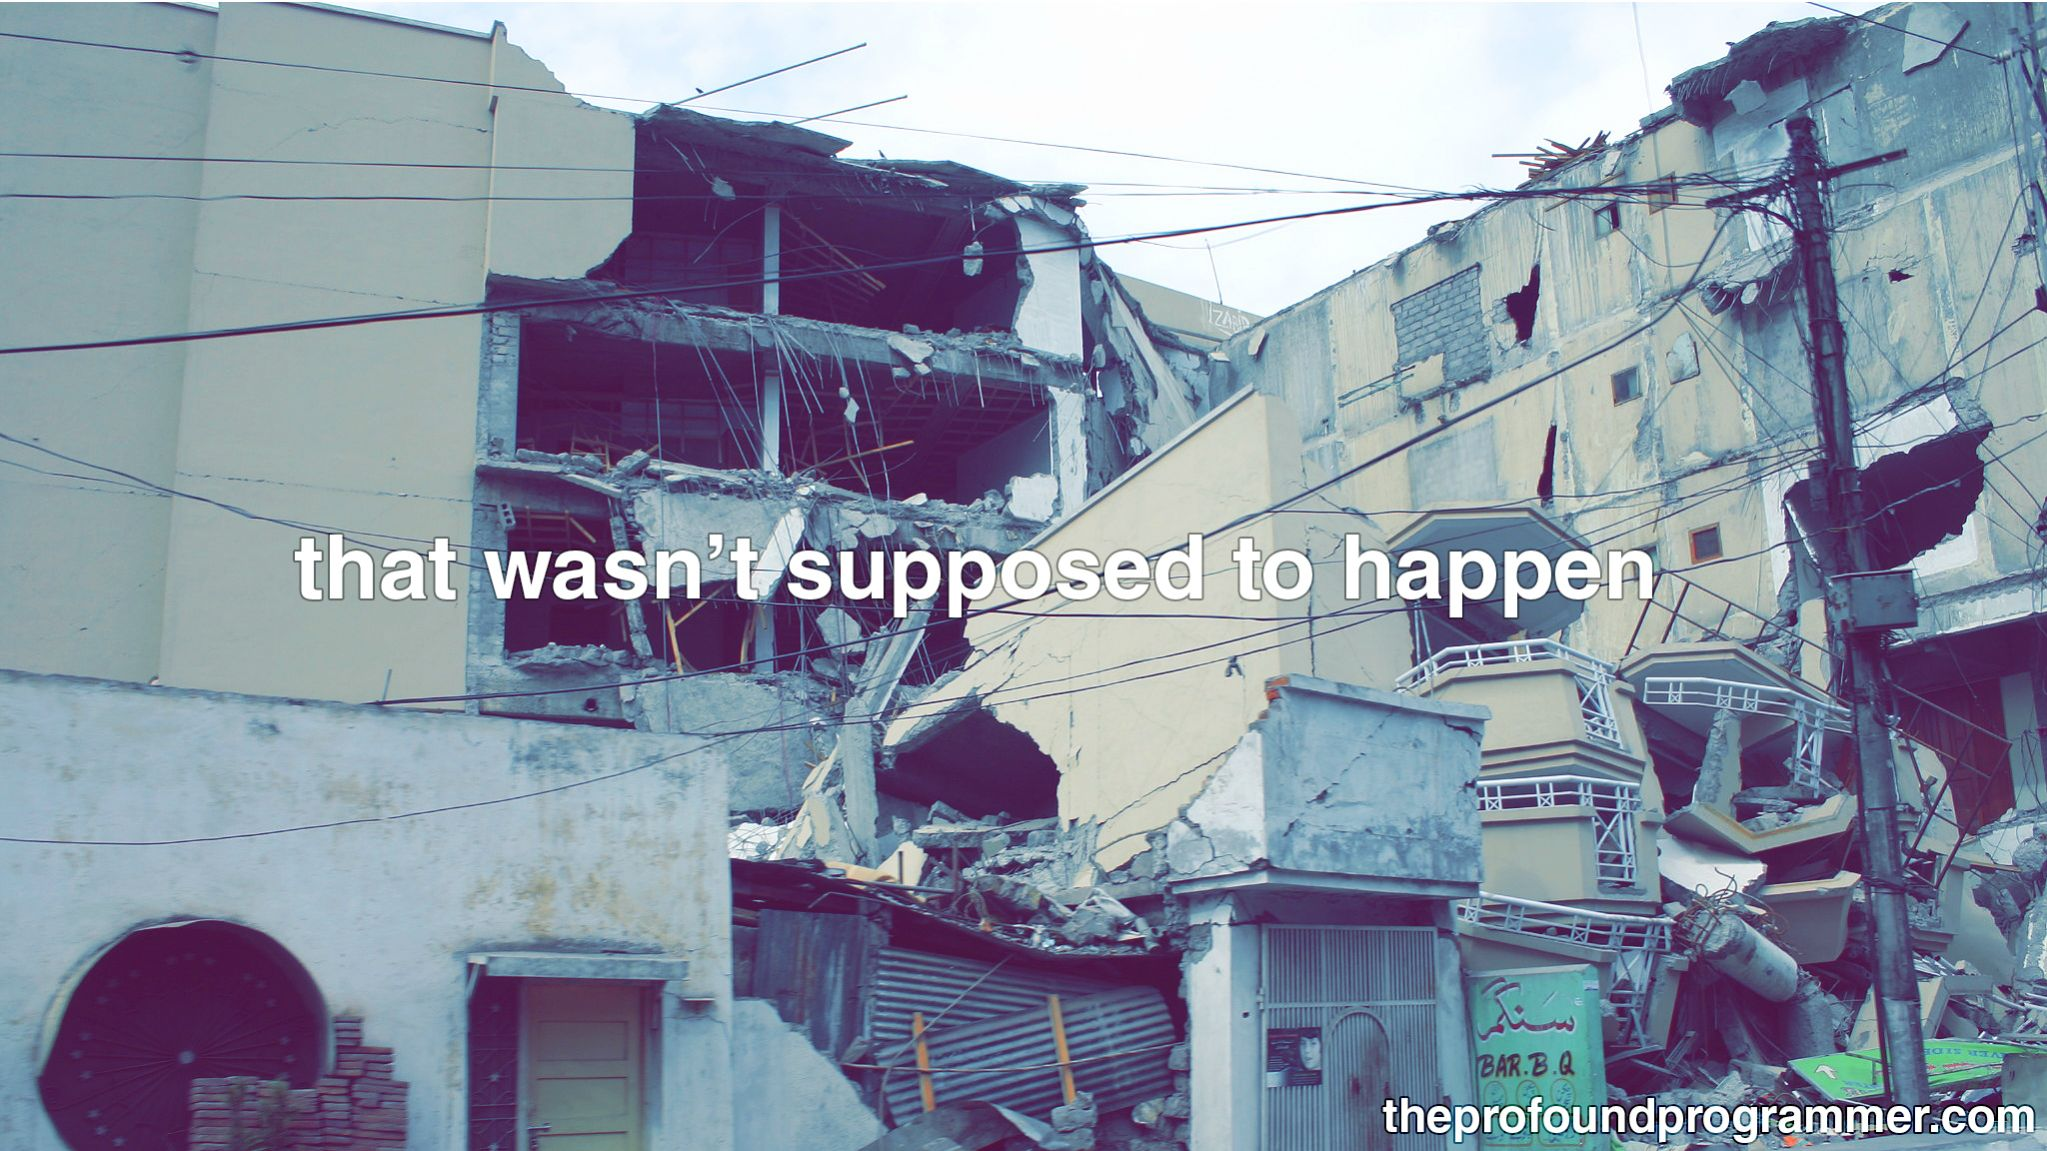
\includegraphics[scale=.15]{img/NG8XW8J8GT.jpg}
    \end{figure}
\end{frame}

\begin{frame}{Eclipse IDE}
    body
\end{frame}

\begin{frame}{Checkstyle}
    body
\end{frame}

\begin{frame}{Fragen ?}
    \begin{figure}
        
\includegraphics[scale=.6]{img/additionalquestions.jpg}
    \end{figure}
\end{frame}

\begin{frame}{Bis nächste Woche !}
    \begin{figure}
        
\includegraphics[scale=.6]{img/dilbert-software-demo.jpg}
    \end{figure}
\end{frame}

\backupend

\end{document}
